\documentclass[master.tex]{subfiles}

\begin{document}

\section*{B. Preliminary}

\subsection{Prospective memory linking window is longer than retrospective
  linking window for a negative memory}

\begin{wrapfigure}{r}{0.5\textwidth}
  \centering 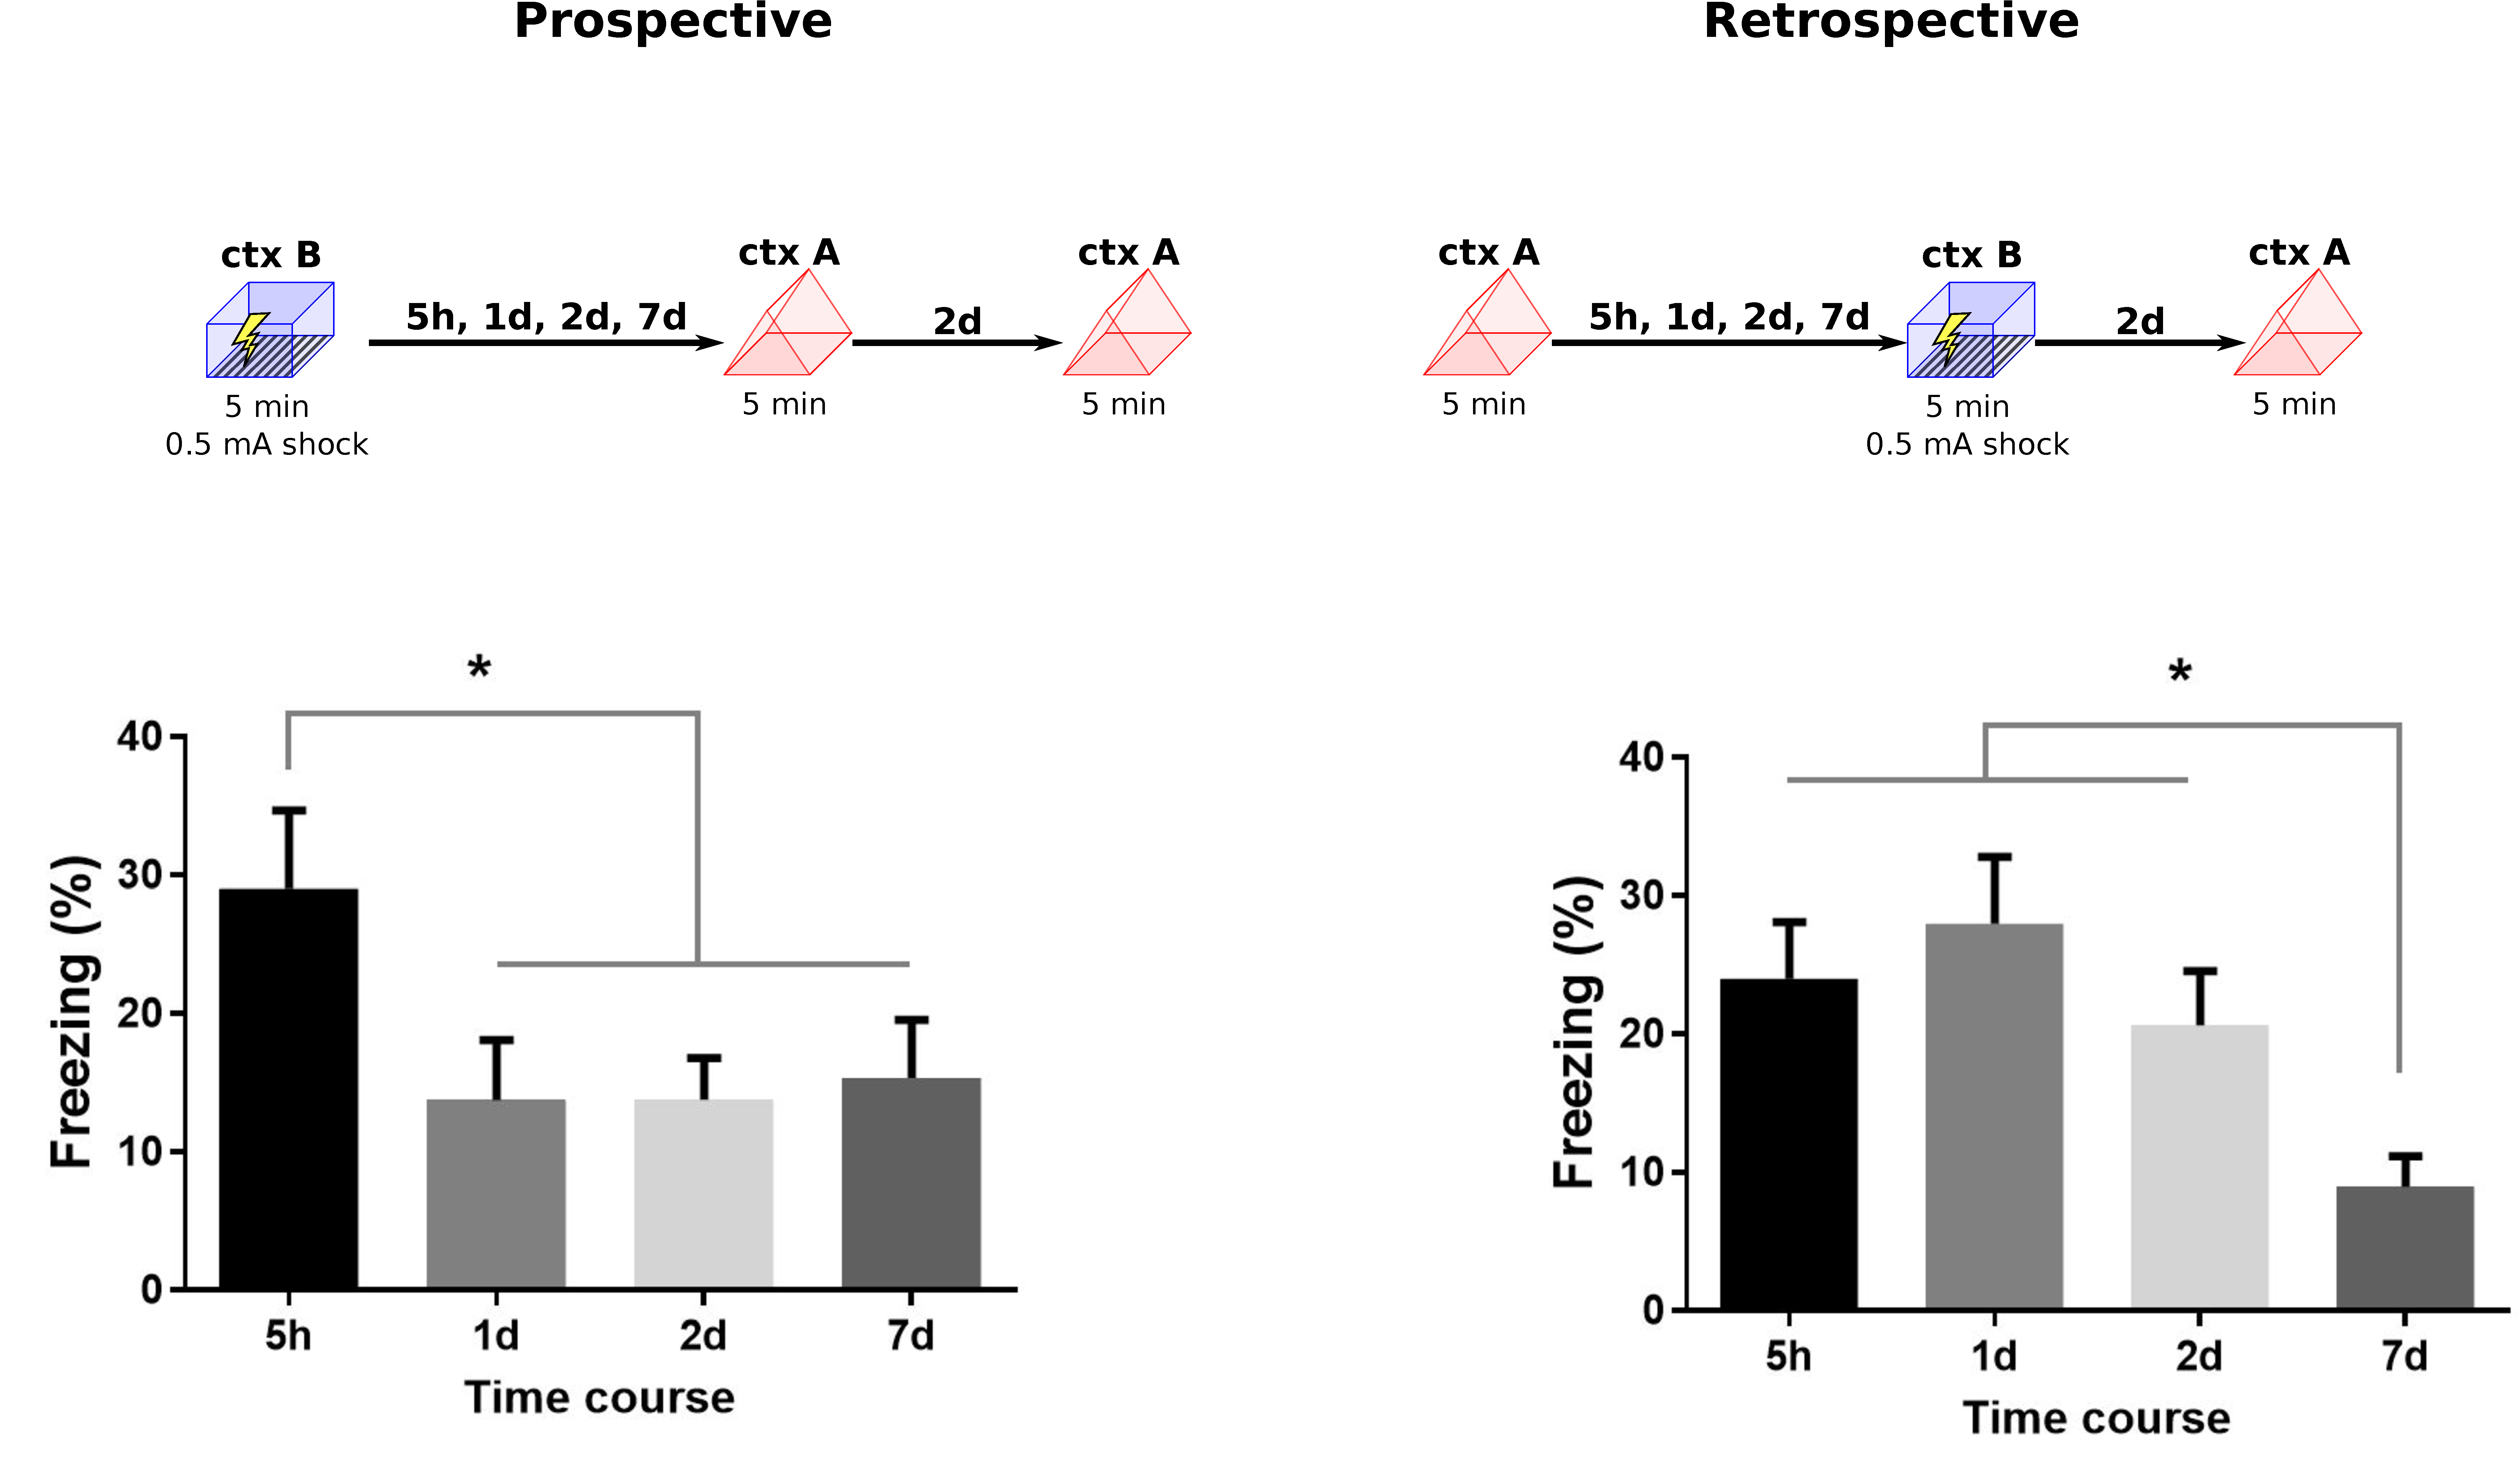
\includegraphics[scale = .4]{Figures/pro_retro_prelim.pdf}
  \caption{\footnotesize Prospective memory linking window is longer than
    retrospective linking window for a negative memory}
  \label{fig:prelim_pro_retro}
\end{wrapfigure}

In the preliminary study, animals are put into two distinct contexts separated
by various time intervals. In the ``prospective linking'' group, animals
received a delayed shock in the first context, and then explore and get tested
in the second context. In the ``retrospective linking'' group, animals explored
first context, and then get a delayed shock in the second context, and then put
back to the first context for testing. Elevated freezing level in the testing
context, where no shock ever occurred for both groups, indicate a transfer of
fear and a linking of the two contexts. For both groups, the exploration and
testing session last 10 minutes, a shock of 0.75 mA was delivered at fifth
minute. The various time intervals are 5 hours, 1 day, 2 days and 7 days for
both groups.

In prospective linking group, we observed a significant higher freezing level in
testing context with 5 hours interval, but not with either 1 day, 2 days or 7
days interval. This suggest that the fear memories were able to transfer forward
to a neutral context 5 hours in the future. On the other hand, in retrospective
linking group, we observed higher freezing level with either 5 hours, 1 day or 2
days interval, but not with 7 days interval. This suggest the fear memory was
able to transfer backward up to 2 days. Taken together, these results suggest an
extended temporal window of retrospective memory linking comparing to
prospective memory linking.

Previously it has been shown that two neutral contextual memories separated by 5
hours interval have significantly larger overlaps in ensemble cells comparing to
those separated by 2 days or 7 days. Furthermore, subsequent fear conditioning
in second context induce significant elevated freezing level in the first
context when the two contexts are separated by 5 hours, but not when they are
separated by 2 days or 7 days. These results suggest that the time window of
memory linking extends beyond 5 hours, but is shorter than 2 days.

We have preliminary results showing that when the second context is paired with
fear during encoding, the time window of memory linking extends to 2 days.
Specifically, when the animals received a delayed shock in the second context
during encoding, there is higher overlap in ensemble cells between the first and
second context during the retrieval test comparing to a ``chance'' level of
overlap between one of the two context and another novel context, even when the
two context are separated by 2 days. Whereas when the second context remains
neutral during encoding, and subsequently associated with fear by an immediate
shock, the ensemble overlap between the two contexts remained at a low level,
consistent with previous findings.

The proposed experiments differ from preliminary studies in two important
aspects: Firstly, the proposed experiments include various time-points within
each group. This enable us to compare freezing level during retrieval testing
and identify the temporal window of memory linking within group, after which the
time window can be compared across group. The advantage for the within-group
design is that we no longer have to compare freezing level across groups,
especially when we are essentially adopting different fear conditioning paradigm
for the two groups which may confound the interpretation of difference in
freezing levels across group; Secondly, the proposed experiment divide each
group into subgroups and test freezing levels in parallel, since the previous
repeated testing paradigm might introduce confounding extinction effects,
especially when we expect memory linking between some of the contexts.

Still, the interpretation of the behavioral data of the proposed experiment
could suffer from another confounding factor \textemdash{} the time interval
between the shock and the encoding of different contexts. An alternative
interpretation of the expected behavior results would be that in ``negative''
group, the freezing level in context B is higher than those in A simply because
the encoding of B happened closer to the shock, and thus associated stronger
with the shock than A, regardless of memory linking, while such time-dependent
associations decays non-linearly across time so that in ``neutral'' group the
freezing levels in B and A are indistinguishable. However, such interpretation
can be distinguished by the analysis of neuronal data, since if the shock is the
driving factor of the observed behavior, there is no reason to expect the
temporal location of the shock affect the ensemble overlaps between either A and
S, B and S, or C and S. Thus the specific hypothesis of the effect of affective
valence on memory linking can still be tested by the proposed experiments.

We have preliminary results showing that when fear conditioning is carried out
in the second context, the fear could transfer back to the first context when
the two contexts are separated by either 5 hours or 1 day, but not when they are
separated by 2 days or 7 days. However, if the fear conditioning is carried out
in the first context, the freezing may transfer to the second context only when
the two contexts are separated by 5 hours, but not when separated by 1 day, 2
days or 7 days. This result suggest a shorter prospective memory linking window.


\end{document}
